% !Mode::"Tex:UTF-8"

\documentclass[a4paper]{article}
\usepackage{ctex}
\author{刘军(NUFE,210042)}
\date{}
\title{Rapid Discrimination of apple essence base on PCA-CH-SVM  }
\usepackage{amssymb}    %使用宏包{美国数学协会符号}
\usepackage{amsmath}
\usepackage{multirow}
\usepackage{tabularx}
% 页面设置
\usepackage[top=2.54cm,bottom=2.54cm,left=3.18cm,right=3.18cm]{geometry}
% 页眉页脚设置
\usepackage{fancyhdr}
\pagestyle{fancy}
\lhead{Rapid Discrimination of apple essence base on PCA-CH-SVM}
%\chead{\thesection}
\cfoot{\thepage}
% 插图包,两个图并排
\usepackage{graphicx}
\usepackage{subfigure}

\begin{document}
\maketitle


Abstract:using new samples to improve the accurate and speed of classification for essence such as apple essence is a key aspect for rapid and accurate determination in online test.In this paper,a novel method for SVM classification ,which extends the traditional SVM method with Principal Component Analysis method and convex hull algorithm to construct the PCA-CH-SVM model,combined with Raman spectra for fast discrimination of apple essence.In this regard,PCA-CH-SVM built on a convex hull of support vectors and new Raman spectra data to classify the apple essence based on features obtained from Raman spectra.The classification model have been evaluated with 10-fold cross validation.The results from this study demonstrated that our approach has good classification accuracy while the training is significantly faster than normal SVM classifiers.



Key words:Apple Essences;Convex hull vector; SVM ; rapidly discrimination
%=============第一部分 简介===================
\section{I. Introduction}
    % 苹果香精检测的背景、
Essence is widely used as a food additive in food industry.Rapid identification of essence for the food industry's quality control is of great significance.The detection of essence is is carried out by physical-chemical indexes and sensory evaluation.sensory evaluation is the traditional and most commonly used method,but its accuracy and objectivity cannot always be ensured because sensory evaluation staff’s judgement can affected by their health condition, emotions, and the environment.

Other methods  are chemistry-based methods such as gas chromatography, mass spectrometry, and gas chromatography-mass spectrometry [5–8].These methods are highly reliable because they use a complete component-by-component approach.However, their shortcomings include excessive test items, being time-consuming,complicated operation, and low capability for insitu and online measurements $^{\cite{Jing, Y}}$. Overall, developing a novel, rapid and reliable method to identify  essence is of positive significance.

Interaction of light with matter gives rise to different types of spectroscopic techniques based on scattering, absorption, reflection and fluorescence.Raman spectroscopy is one such technique which is arising from inelastic scattering of laser light by the molecular vibration inside the sample. As a result, the scattered photons are emitted with the different frequency (energy). This difference in frequency between incident and emitted protons provides finger print about the rotational, vibrational and other low frequency transitions in molecule. Thus Raman spectrum, which is the plot of intensity as function of Raman shift, is a rapid detection method developed in recent years, with fast, efficient, non-polluting, without pre-treatment, lossless analysis, etc., many areas have been widely used.[拉曼在食品检测中的文献]

Support Vector Machine (SVM) $^{\cite{Vapnik}}$ has been successfully used for for data mining, pattern recognition and artificial intelligence fields [2–5]. With labeled data, SVM learns a boundary (i.e., hyperplane) separating different class data with maximum margin.
The classification process usually face the new evolving data,the initial training sample set can not reflect all the sample information.When new training samples are accumulated to a certain scale, in order to obtain the new sample information,it would like to integrate these examples and train a new classification model.However, the training of a SVM has the time complexity of $O(M^3)$(M is the number of training samples), it does benefit large-scale online applications.

To attack this problem,lots of works have been done.One way is to reduce training samples with a certain sample selection strategy.The quality of training data set is vital to the performance of the classifier being constructed.Syed et al.$ ^{\cite{Stefan}}$ worked out an incremental algorithm based on SVM, which retains only the support vector set as a historical training sample.

This paper selected apple essence as sample to study a novel PCA-CH-SVM method based on Raman spectra to rapid and reliable classify essence.
%=============第二部分 实验与材料===================
\section{II.Experiments and Materials}
\subsection{Sample collection and preparation}
A total of 27 experimental samples, corresponding to 3 apple essence brands,were obtained from three famous flavors and fragrances companies in China by three batches.All samples were produced in 2016,and had equivalent proofs.The apple essence included in study are listed in Table1.

The overall procedure of sample collection is same. In total,Raman spectra of 300 samples of 3 apple essence brands have been used in this study.Out of 300 samples,xx were

Essence contains a large number of volatile, low content components.The complex pretreatment methods of samples have some impact on these components.In order to avoid introducing other impurities or the distortion of component proportion caused by improper pretreatment method,in this experiment, the test samples are prepared by high dilution of pure water.Add 3 grams of essence in the volumetric flask,was respectively diluted 10 times and 1000 times with high purity water,and  shaked well, then got samples.The  standard  safety  rules  have  been  followed  at  each step from sample collection till acquisition of Raman spectra。

%\left(
%  \begin{array}{Detailed information of the investigated apple essences}
%    flavor companies & no. & solvent \\
%    A & S & ethanol \\
%  \end{array}
%\right)

\begin{table}[h] %开始一个表格environment,表格的位置是h,here
  \centering
  \caption{Detailed information of the investigated apple essences}\label{a}
  \begin{tabular}{c|c|l}

     \hline
     % after \\: \hline or \cline{col1-col2} \cline{col3-col4} ...
     flavor companies       & no.       & solvent \\
     \hline
     \multirow{3}{*}{A}       & S         & ethanol \\
     \cline{2-3}
                              & Q         & ethanol \\
     \cline{2-3}
                              & I         & 1,2 propanediol \\
     \hline
     \multirow{3}{*}{B}       & a         & 1,2 propanediol \\
     \cline{2-3}
                              & b         & ethanol,1,2 propanediol \\
     \cline{2-3}
                              & c         & 1,2 propanediol,water \\
     \hline
     \multirow{3}{*}{C}       & d         & 1,2 propanediol \\
     \cline{2-3}
                              & e         & ethanol \\
     \cline{2-3}
                              & f         & 1,2 propanediol \\
     \hline
   \end{tabular}

\end{table}



\subsection{Raman spectrum acquisition}%拉曼光谱的获得
Raman spectrum for all samples have been acquired with Raman spectrometer(Prott-ezRaman-d3,Enwave Optronics, USA).Raman  signal  is  normally  very  weak  as  compared  to  Rayleigh  scattering,  therefore  an acquisition time of 10 seconds has been used for recording each spectrum.The spectrum from the  sera  samples  have  been  recorded  in  the  spectral  range  of  250 $cm^{−1}$  to  2350 $cm^{−1}$,  as  it contained the most useful information.

\subsection{Data analysis and processing}%
Raman  spectrum  of  essence samples  is  normally  very  complex  and  rich  of  chemical information.  Since  in essence  samples,  there  exist  different  types  of  functional group compound. The Raman spectrum of each of these compound consists of  numerous peaks.  The  visual  assignment  of  any  particular  peaks  to  a  specific  molecule usually  produces  imprecision  in  the  final  result,  because  most  of  the  time  different molecules  contribute  to  the  same  peak.  In  order  to  overcome  this  limitation  of  visual analysis, statistical methods are mostly used for the interpretation of Raman data of essence samples. With the statistical approach one can extract useful information from the data set by high  lighting  the  similarities  and differences.  In  this  study,  we  are using convex hull SVM  for  the  classification of  apple essence,  in order to efficiently handle large amounts of sample data.

Principal components analysis(PCA)  is  a  method  for  the  re-expressing  multivariate  data.   It  allows  the researcher to reorient the data so that the first few dimensions account for as much  of  the  available  information  as  possible.  The  principal  components solution has the property that each component is uncorrelated with all others, which  has  the  advantage  of  eliminating  multicollinearity.

The number of the generated features was still quite large for  the  classifier.  So  PCA  was  used  to  perform  feature reduction  before  pattern  recognition.  Then  standard soft-margin  C-SVM  was  used  for  classification  of  Chinese liquors.

\subsection{Incremental SVM Learning Base on Convex Hull Vector}
In the formulation of a SVM,we find that in feature space the decision surface is always an hyerplane,and the classifier is always written in terms of data instances that belongs to the outside of the boundaries of the classes.More secifically,in the separable case,the boundaries of classes contain the instances of solution(support vectors),therefore we only need the points on those boundaries.The boundaries of the data can be obtained from the Convex Hull of each class.In particular,we only need the extreme points(vertices) of the Convex Hull.


%Once every class convex hulls are represented by samples, the separating hyperplane can be constructed by the nearest point problem. A convex hull of a class can be convex combined by boundary samples or vertices of the convex hull. So using those boundary samples or vertices to train SVM will be equivalent to using all training samples to solve the normal SVM problem.



\begin{figure}[h]
  \centering
  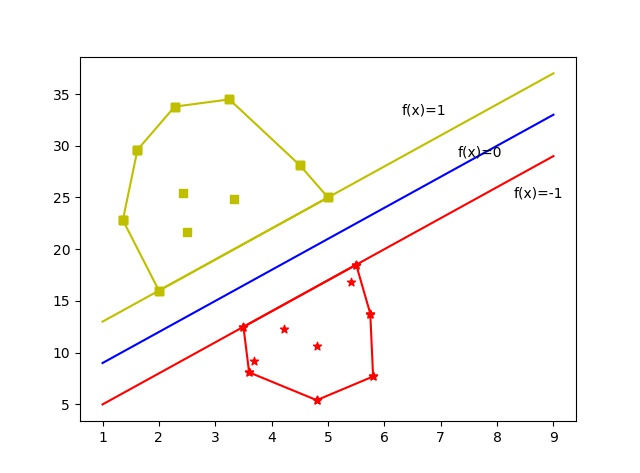
\includegraphics[width=9cm,height=6cm]{HullVector_SupportVector}
  \caption{Relationship between hull vectors and support vectors}
\end{figure}

The convex hull(CH) of a set of points S is the minimum convex set that contains S.Mathematically,CH is defined as:
$$
CH(X) :\{ \omega = \sum_{i=1} ^{n} \alpha_i x_i, \alpha_i \geq 0, \sum_{i=1} ^{n} = 1, x_i \in X \}
$$

Basically SVM classification can be grouped into two types: linearly separable and linearly inseparable cases. The nonlinear separation can be transformed into linear case via a kernel function to transform the original space to a higher-dimensional space, and a hyper plane is constructed in the higher-dimensional space to solve problems of nonlinear separable classification in the original low-dimensional space.
 
 In linear separable case:existing history training data set X,it can be divided into two categories: $X^{+}$ and $X^{-}$
$$
CH(X^{+}) \bigcap CH(X^{-}) = \varnothing
$$
\begin{figure}[h]
  \centering
  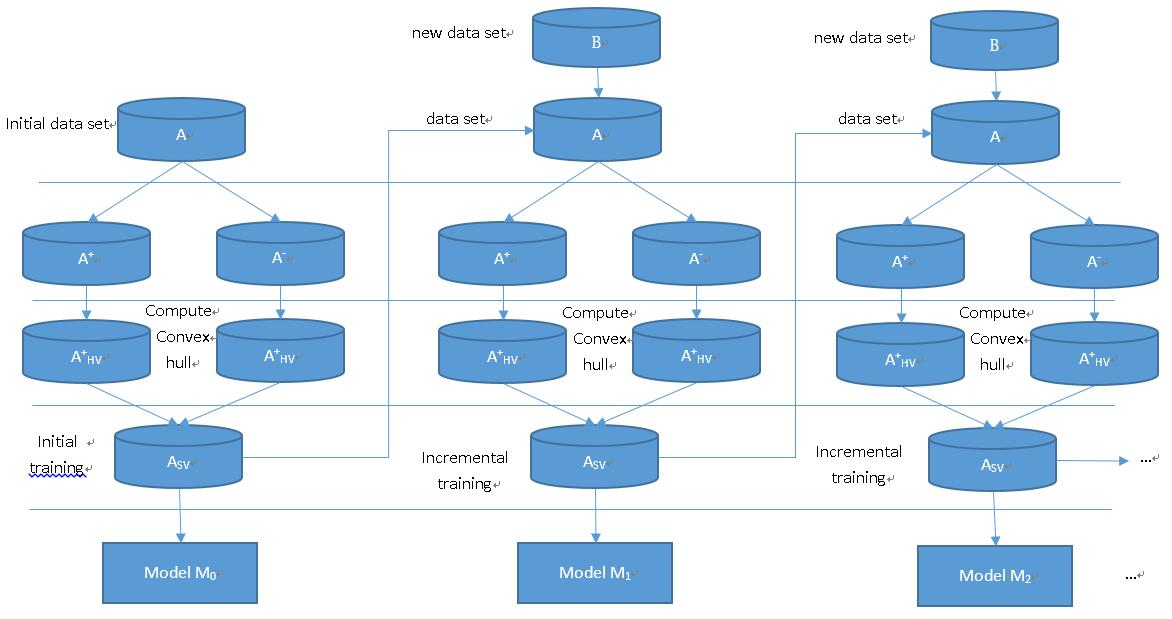
\includegraphics[width=9cm,height=6cm]{算法示意图}
  \caption{Gneral process of the method}
\end{figure}
In this work,a Convex Hull SVM algorithm was attempted for classification due to its good incremental learning.The procedure is summarized as follows:\\
\begin{enumerate}
\item for data set$A^{+}$ and $A^{-}$,Compute the convex hull vector set $A ^{+}_{H_{V}}$ and $A^{-}_{H_{V}}$, $A_{H_{V}} = A ^{+}_{H_{V}} + A ^{-}_{H_{V}} $
\item use $A_{H_{V}}$ as train data set, train SVM model,and get support vectors $A_{S_{V}}$ \\
\item add the new train data set B,make $A = B \bigcup A_{H_{V}}$ as new train data set,get new $A^{+} = A^{+} _{H_{V}} + B^{+}$ and $A^{-} =  A^{-} _{H_{V}} + B^{-}$,then calculate the new hull vector set  $A_{H_{V}} = A ^{+}_{H_{V}} + A ^{-}_{H_{V}} $\\
\item as hull vector set $A_{H_{V}}$ as train data set to train SVM model,and get support vector set $A_{S_{V}}$ ,then get the classifer.    
\end{enumerate}

1.for data set$A^{+}$ and $A^{-}$,Compute the convex hull vector set $A ^{+}_{H_{V}}$ and $A^{-}_{H_{V}}$, $A_{H_{V}} = A ^{+}_{H_{V}} + A ^{-}_{H_{V}} $
2.use $A_{H_{V}}$ as train data set, train SVM model,and get support vectors $A_{S_{V}}$ 
3.add the new train data set B,make $A = B \bigcup A_{H_{V}}$ as new train data set,get new $A^{+} = A^{+} _{H_{V}} + B^{+}$ and $A^{-} =  A^{-} _{H_{V}} + B^{-}$,then calculate the new hull vector set  $A_{H_{V}} = A ^{+}_{H_{V}} + A ^{-}_{H_{V}} $
4.as hull vector set $A_{H_{V}}$ as train data set to train SVM model,and get support vector set $A_{S_{V}}$ ,then get the classifer.
Repeat steps 3) and 4 enable continuous incremental learning of new samples.

%=============第三部分 数据分析===================
\section{III. Data Analysis}
% 拉曼数据分析
\subsection{Raman spectrum Data analysis}
Raman spectroscopy can quickly obtain sample information about the functional groups in aromatic compounds,and has significant advantages: sample preparation is simple, measurement usually does not destroy sample, and moisture does not affect test.

Raman spectrum of Apple essence samples is normally very complex and rich of information of functional group of organic compounds.The Raman spectra mainly reflected the solvent information of the essence, and the Raman spectra of the essence with the same solvent are extremely similar and difficult to be identified manually,as shown in Figure 1.The spectra of essences e, Q, and s are similar,and i,a,c,d,f is similar.The spectra B has more peaks,and contains the peaks of the previous two types of spectra.According to the literature[23] and comparison of standards,the spectra of essences e, Q, and s are the peak of

%=============第四部分 结果与分析===================
\section{IV. Result and Discussion}
The  model  takes  the  whole  Raman  spectrum  and  selects  discernable  features  from the  spectrum.  Later  on  the  model  uses  those  features  for  predicting  unknown  samples.  The developed model has been evaluated by using 10-fold cross validation approach. It basically divided  the  whole  data  set  into10-subsets.  Each  time  the  model  is  trained  on  9  subsets  and tested  on  the  remaining  one.  The  overall  process  is  repeated  10-times,  to  predict  all  the samples stepwise. The beauty of this method is that it does not care about how the data set are divided, because each data must come k-1 times in the training set and once in test set.
\begin{figure}[h]
  \centering
  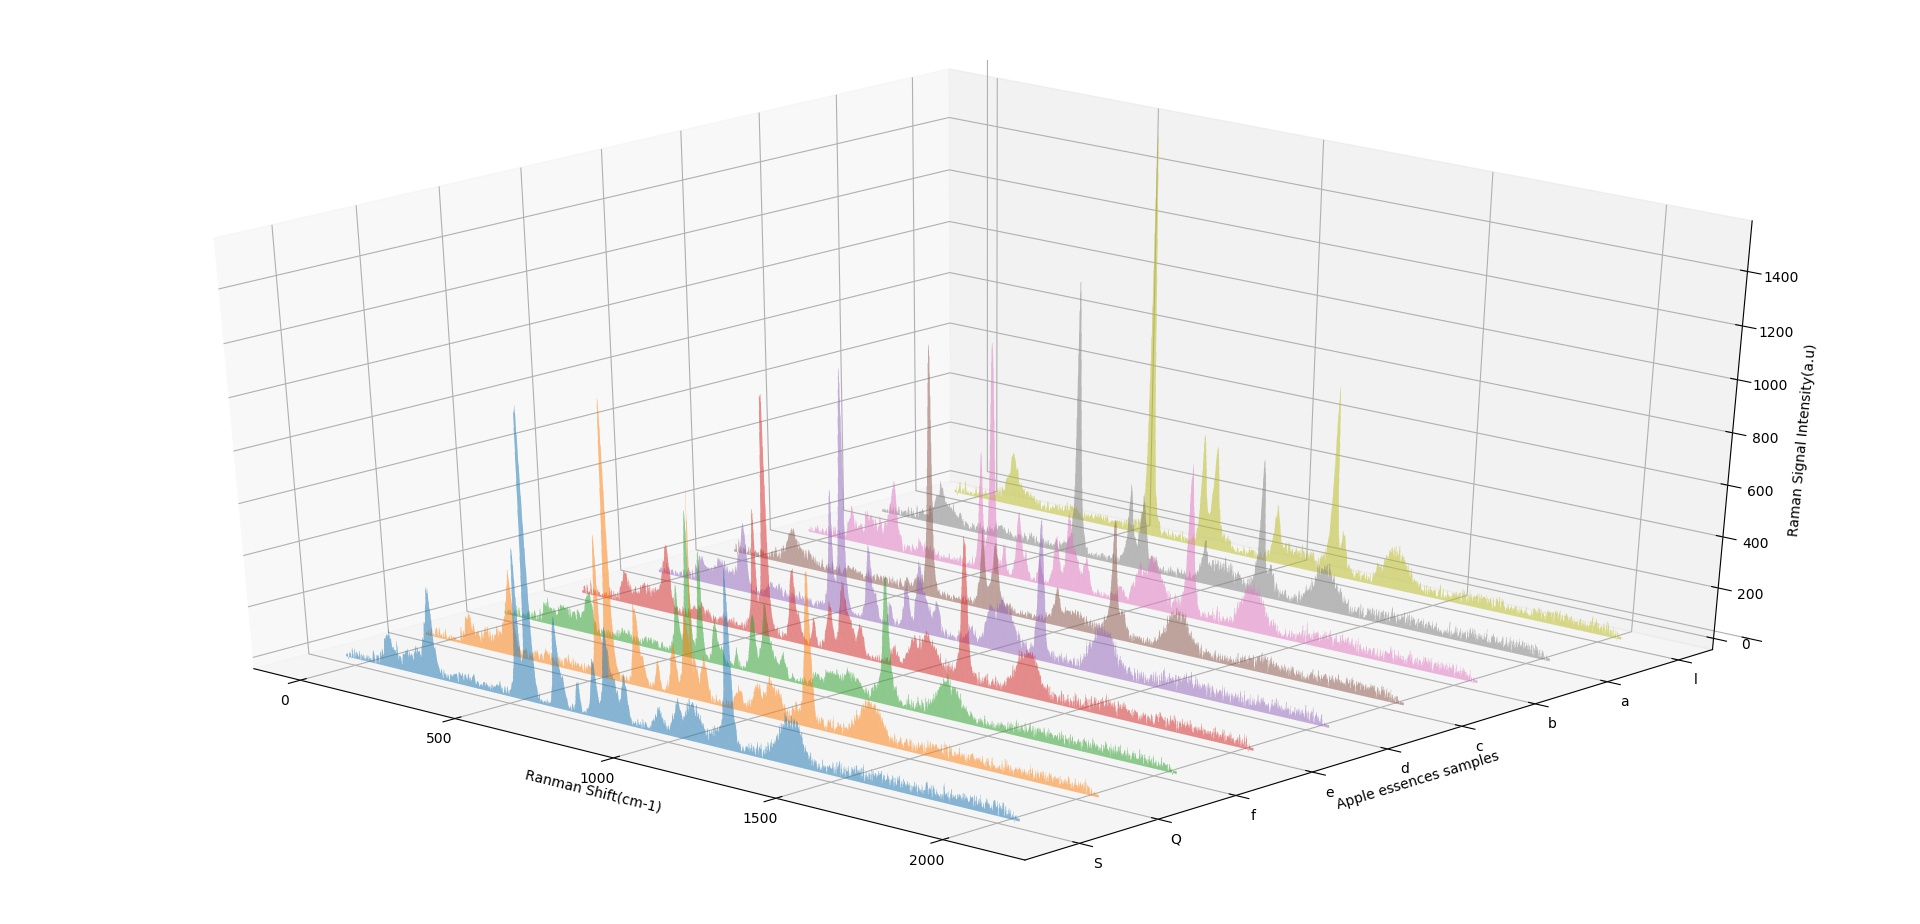
\includegraphics[width=9cm,height=6cm]{Typical_Raman_spectra}
  \caption{Typical Raman spectra of nine kinds of apple essences}
\end{figure}
The overall results for the model with different kernel functions are given in Table 1. The best  performance  has  been  obtained  with  the  polynomial  kernel  function  of  order  1.  The performance  of  a  model  is  usually  evaluated  in  terms  of  accuracy,  precision,  sensitivity  and specificity.  Sensitivity  correctly  sorts  out  all  patients  with  the  disease,  whereas  specificity correctly identifies all patients who do not have that disease [29]. A laboratory test with high specificity and sensitivity is usually desired, but rarely both of these conditions are met at the same time. The aforementioned four parameters for the current SVM model with polynomial kernel function of order 1 have been found 85%, 90%, 73% and 93%, respectively.

%不同香精中化学成分及相对含量不尽相同,组分化合物间也会发生不同的缔合作用,
The chemical components and relative contents of different flavors are different,these will produce different associations,so it  determine the spectral curves of different flavors are somewhat different,and has different  characteristics and fingerprints.The difference between the spectra is the variation of relative intensities of the absorption peaks in the fingerprint region,and the Minute difference in the small peaks in the fingerprint region.Pattern recognition algorithm can maximize the information extracted from the data,and can classify the sample set.



For comparison, three different algorithms were simulated.Algorithm A uses the standard SVM algorithm, which uses all the samples to solve the support vector for each incremental learning.Algorithm B uses the support vector set instead of the original sample set for incremental learning,Algorithm 2 uses the support vector set instead of the original sample set for incremental learning, that is,using the original classifier support vector set instead of the original sample set, combined with the new sample to be calculated together.Algorithm 3 is a shell vector incremental learning algorithm.The initial sample set is 135 samples randomly selected from all samples, and 70 samples are added for each incremental learning. After each learning, using all 345 samples to check the classification effect.The results are shown in Table 2,after the first to third incremental learning process,Compared with the new shell vector set, the number of shell vectors transformed into non-shell vectors is 14,17,18.



It can be seen from the simulation results that the SVM incremental learning algorithm based on shell vector is compared with the standard SVM method, which greatly saves the computation time and accelerates the simulation speed, and the classification accuracy is basically the same,the algorithm, that combined the original support vector set with the new sample set rather than an initial sample set,greatly saves the computation time and accelerates the simulation speed, and the classification accuracy is basically the same.Meanwhile, with the continuous learning of incremental learning, the algorithm can naturally make part of the Hull vector into non-Hull vector, to achieve the selective forgetting of the historical data of the training.Therefore, when dealing with a large number of online data set ,the speed advantage of the incremental hull SVM method is more obvious.

\begin{table}[h] %开始一个表格environment,表格的位置是h,here
  \centering
  \caption{Simulation results after adding group samples}\label{a}
  \begin{tabular}{|p{3.5cm}|c|p{1.5cm}|c|c|c|c|}

     \hline
     % after \\: \hline or \cline{col1-col2} \cline{col3-col4} ...
     learning process       & algorithm       & Simulation sample   & Hv    & Sv & t/s    & $\eta$  \\
     \hline
     \multirow{3}{3cm} {Initialization(randomly selected 135 sample data)}&1    &135 & - &34 & 37.5 & 85.80         \\
                                                                       &2    &135 & - &34 & 37.5 & 85.80         \\
                                                                       &3    &135 & - &34 & 37.5 & 85.80         \\

    \hline
     \multirow{3}{3.5cm}{After the first incremental study(add 70 sample data)} &1    &135 & - &34 & 37.5 & 85.80         \\
                                                                       &2    &135 & - &34 & 37.5 & 85.80         \\
                                                                       &3    &135 & - &34 & 37.5 & 85.80         \\
    \hline
    \multirow{3}{3.5cm} {After the second incremental study(add 70 sample data)} &1    &135 & - &34 & 37.5 & 85.80         \\
                                                                       &2    &135 & - &34 & 37.5 & 85.80         \\
                                                                       &3    &135 & - &34 & 37.5 & 85.80         \\
    \hline
    \multirow{3}{3.5cm} {After the third incremental study(add 70 sample data)} &1    &135 & - &34 & 37.5 & 85.80         \\
                                                                       &2    &135 & - &34 & 37.5 & 85.80         \\
                                                                       &3    &135 & - &34 & 37.5 & 85.80         \\
    \hline
  \end{tabular}

\end{table}

%=============第五部分 结论===================
\section{V.	Conclusion}
This  study  demonstrates  the  use  of  Raman  spectroscopy  combined  with Convex-Hull SVM  technique  for the  classification  of  the  spectral  data  acquired  from  Apple essense. Raman  spectroscopy  coupled  with  statistical  tools  has  great  potential  to  contribute significantly in the On-line inspection and research of product quality in an effective way.There is also a great  likelihood  to  use  Raman  spectroscopy  combined  with  one  of  the  existing  methods  for initial screening in order to increase the inspection efficiency. The results obtained are quite promising and interesting. The research work in our laboratory is still in progress striving for increasing sensitivity as well as specificity.

\renewcommand\refname{References}
\begin{thebibliography}{99}
    \bibitem{Vapnik}V.N. Vapnik, The Nature of Statistical Learning Theory, Springer, New York,1995, 8 (6) :988 - 999
    \bibitem{Stefan}Stefan Ruping,Incremental Learning with Support Vector Machines,Technical Reports,2001,228(4):641-642
    \bibitem{XIAORong}XIAO Rong, WANG Ji-cheng, SUN Zheng-xing. Anapproach to incremental SVM learning algorithm.Journal of Nanjing University, 2002, 38(2): 152 157.
    \bibitem{Zhu X}Zhu X, Lafferty J, Ghahramani Z. Combining active learning and semi-supervised learning using Gaussian fields  and  harmonic  functions[C].  In:  Proc  of  ICML  2003  Workshop  on  the  Continuum  from  Labeled  to Unlabeled Data. Menlo Park, CA:AAAI Press,2003:58-65.
    \bibitem{yunjungShin}Hyunjung Shin, Sungzoon Cho, Invariance of neighborhood relation underinput space to feature space mapping, Pattern Recognition Letters, 26 (2005)707–718.
    \bibitem{YJLee}Y.J. Lee, S.Y. Huang, Reduced support vector machines: a statistical theory,IEEE Transactions on Neural Networks 18 (No.1) (2007) 1–13.
    \bibitem(Jing, Y)Jing, Y.; Meng, Q.; Qi, P.; Zeng, M.; Li, W.; Ma, S. Electronic nose with a new feature reduction method anda multi-linear classifier for Chinese liquor classification. Rev. Sci. Instrum. 2014, 85, 055004. [Cross Ref][Pub Med]

    \bibitem(K.P. Bennett1)K.P. Bennett , E.J. Bredensteiner, Geometry in Learning, Geometry at Work, C. Gorinieditors, Mathematical Association of America, 132-145, 2000
    \bibitem(K.P. Bennett2)K.P. Bennett , E.J. Bredensteiner, Duality and Geometry in SVM Classifiers, 17thInternational Conference on Machine Learning, San Francisco, CA, 2000
\end{thebibliography}


\end{document}

